
Grand united theories \cite{bib:patisalam},
composite models \cite{bib:composite}, technicolor \cite{bib:technicolor},
as well as superstring-inspired $E_6$ models \cite{bib:e6} 
are all well-motived theories   
that
postulate the existence a symmetry, beyond the $SU(3)_C x SU(2)_L x U(1)_Y$
of the standard model (SM)\cite{bib:sm}, 
that relates quarks and leptons and that would
imply the existence of new bosons, called leptoquarks (LQ).
A LQ is colored, has fractional electric charge, can
be spin 0 (scalar LQ) or spin 1 (vector LQ),
and couples to a lepton and a quark with coupling strength
$\lambda$.  
A LQ  
decays to a charged lepton and a quark (with unknown branching fraction
$\beta$) or a neutrino and a quark (with branching fraction
$1-\beta$).

Constraints from experiments sensitive to flavor changing
neutral currents, lepton family-number violation,
and other rare processes\cite{bib:lqconst}
exclude LQ's with masses accessible to current collider experiments
that couple to more than one quark/lepton generation.  
They also constrain
the coupling constant $\lambda$ at these masses to be less than 0.3.

This paper presents the results of a search for a first-generation LQ
using a data sample corresponding to 50 \ipb~ taken with the CMS
detector during December, 2009 
at the CERN LHC \pp~ collider operating with \sqrts = 10 \tev~ using
events containing two electrons and two jets.
The average instanteous luminosity during this run was $5 x 10^{34}$
with a mean number of \pp~ interactions per crossing of 17.
Current limits from the CDF \cite{bib:cdflq}
and D0 experiments \cite{bib:d0lq}
constrain the mass of a first generation scalar LQ to be $>$ 236 \mgev.

In \pp~ collisions at \sqrts = 10 \tev, LQ's are predominant pair-produced 
via gluon gluon fusion with a production
cross section that is determined by the strong coupling
constant $\alpha_s$ and that is independent of $\lambda$.
The cross section depends on the spin and the mass
of the LQ and has been calculated to
NLO \cite{bib:kramer1}.  The uncertainty on the cross section is
dominated by uncertainties on the parton distribution functions
(PDF's) and has been estimated to be 10\%. \cite{bib:kramer2}.

The CMS detector \cite{bib:cmsjinst} consists of a large-bore
superconducting solenoid with a 3T central field 
that encloses the central tracking and calorimeter systems. 
The central tracking system is composed of
an all-silicon pixel and strip tracker that provide efficient
reconstructions of vertices and the momenta of charged particles with 
pseudorapidities \aeta$<2.0$ \cite{bib:geo}.  
A lead-tungstate scintillating-crystals electromagnetic 
calorimeter, and a brass-scintillator sampling
hadron calorimeter are used to measure the momenta of photons,
electrons, and hadrons.
The central calorimeters cover \aeta$<1.4$ and the endcap
calorimeters cover \aeta$<$ 3.0; 
The iron yoke of the solenoid's flux-return 
is instrumented with four stations of muon
detectors cover \aeta$<$2.4.
Forward  sampling calorimeters extend the pseudorapidity
coverage to high values ($\eta \approx 5$) assuring very good hermeticity.
Luminosity is measured using the forward calorimeters 
The normalization is set by a Van der Meer scan and the 
uncertainty is estimated to be 10\%. \cite{bib:lumi}.
Events are stored for offline analysis 
that satisfy one of the 
trigger requirements at a rate of approximately 100 Hz.
Events first must pass a trigger  
from a system of fast electronics that
reconstructs objects within a subsystem (calorimeter or muon) and
that makes
a decision for every beam crossing.  The information from all subsystems
for these events are then processed by a
Higher-Level Trigger (HLT)
that consists of a farm of commercial cpu's that runs a version
of the offline reconstruction optimized for timing considerations.

Events used in this analysis are required to pass a trigger that requires a
cluster of energy in the electromagnetic calorimeter with \et $>$ 10
\pgev~ and that passes a loose requirement on the ratio of hadronic
to electromagnetic energy and shower shape requirements on
the trigger tower in cluster containing the highest energy
in the first level trigger and
15 \pgev~ in the HLT.

Electron candidates, reconstructed offline, are required to have 
a reconstructed electromagnetic cluster with
transverse energy
($\et$) $>$ 25 \pgev, \aeta$< 2.5$, and must be 
spatially matched
to a reconstructed track in the central tracking system. 
(\et~ is calculated using the energy
from the calorimeter and angles from the matched track.) 
Electron candidates are further required
to have a shower shape consistent with that of an electromagnetic shower 
and be isolated from other energy deposits
in the calorimeter and from 
reconstructed tracks in the central tracking system.
Only the two highest \et~ electrons in the event are considered
in this analysis.
At least one of these two 
must be well-matched to the HLT electron that triggered the event. 
The energy scale is set using \zee~ and $\pi_0$ events.
For electrons within the fiducial region of the calorimeter and with
\et $> 25$ \pgev, the average reconstruction efficiency is
measured to be 95\%
by comparing the rate of \zee~ events, after background subtraction,
with two electrons, and
with only 1 electron, passing the full identification requirements.
Due to a small gap between the barrel and endcap calorimeters at
\aeta $\approx$ 1.5 and the reduced tracking efficiency beyond
\aeta~ of 2.0, the efficiency times geometric acceptance for
electrons is approximately 0.8.
More details on the electron selection can be found in
\cite{bib:cmseid}


Jet are reconstructed from the calorimeter energies using an 
iterative cone algorithm.  The jet energy scale is determined using
a combination of dijet events and $pp \rightarrow \gamma + {\rm jets}$ events.
The jet energy resolution is measured using dijet events.
More details on the jet reconstruction and calibration
can be found in
\cite{bib:cmsjetid}.  Jets that are within a cone of size
$\Delta R=\sqrt{\Delta (\eta^e-\eta^j )^2 + \Delta(\phi^e-\phi^j)^2}=0.3$
of one of the two highest \et~ electrons
passing the ID requirements
are removed from the jet list.
In this analysis, only jets with \et $>$ 25 \pgev~ 
and \aeta $<$ 3.0 are considered.
Only the two highest \et~ jets are used in the subsequent analysis.

Muons are used as part of our data-based evaluation of backgrounds
from standard model processes.  Muons candidates are
constructed from a track
reconstructed in the central tracking system with a good match
to a reconstructed track in the muon system.  Muons used in this 
analysis are required to have transverse momentum (\pt) $>$ 25
\pgev and \aeta $<$ 2.0.  The muon reconstruction efficiency
is measured in data using \zmumu ~ events.


We select an initial sample containing two electrons and two jets.

The dominant SM processes that produce such events 
are \ttbar~ and \zee+jets~ production.  Other backgrounds 
include multijet production with at least 2 jets misidentified as
electrons, W+jets events with a jet mis-identified as an electron,
and multi-boson production.  
To reduce these backgrounds, 
we require both electrons have \et $>$ 30 \pgev, and 
both jets have \et$>$ 50 \pgev.
To reduce from \zee~ production, we require the invariant mass of the
electrons to be $>$ 100 \mgev.
To further reduce all SM backgrounds,
we require \st, defined as the
scalar sum of the magnitudes of the \pt~ of the electrons and jets.
The value of the \st~ requirement depends on the LQ mass and is given
in table~\ref{tab:lqeff}.
The cut value was chosen as the one that is predicted to
give the optimum signal significance.

The acceptances times efficiency for pair-production
of scalar LQ's 
in given in Tab. ~\ref{tab:lqeff}, and is evaluated 
using Monte Carlo LQ events produced with the PYTHIA\cite{bib:pythia}
event generator and a detector simulation based on
GEANT\cite{bib:geant}, 
overlaid with events collected by
the CMS detector without any trigger requirement
(to simulate the effects of other \pp~ collisions in the same
crossing and detector noise).
A small correction (O(xx\%)) to $e\cdot A$ is applied 
based on the electron identification efficiencies measured using
\zee~ events and jet resolutions measured using dijet events.


\begin{table}
\begin{center}
  \begin{tabular}{| l | c | c | c | c | } \hline
   mass (\mgev) & \st~  cut & LQ A & LQ A $\cdot$ e & number events \\
  \hline \hline
 250 & XX & XX & XX & XX  \\
 350 & XX & XX & XX & XX  \\
 450 & XX & XX & XX & XX  \\
 550 & XX & XX & XX & XX  \\ \hline
  \end{tabular}
    \caption{Acceptance (A) for \lqlqbar~ events to pass the geometric and kinematic
requirements of this analysis, acceptance times efficiency (A$\cdot$e) for passing
the electron and number of expect events in 50 \ipb. }
    \label{tab:lqeff}
\end{center}
\end{table}    

The \ttbar~ background is evaluated both using MC
(MADGRAPH ~\cite{bib:madgraph} plus full detector simulation)
and using a data-based technique.  
Since the W's produced in \ttbar~ events decay to 
electrons and muons, while LQ decay's are constrained to only
one generation,  events that pass all the LQ selection requirements,
except with one electron and one muon instead of two electrons,
can be used to estimate this background.
The background in the two electron sample is given by
$$B_{\ttbar}=0.5 N_{e\mu} {{e \cdot A (ee)_{MC}}\over {e \cdot A (e\mu)_{MC}}}$$
where $e \cdot A$ is the acceptance for \ttbar~ events as evaluated
using the full MC corrected for the data-derived efficiencies and 
resolutions. 
We observe XXX events in our control sample for an \st~ require
of 460 GeV, for a statistical uncertainty on our background
predicition of XX\%.
The two methods give similar results.

The \zee~ background is also evaluated using both MC
(MADGRAPH plus full detector simulation) and using a data-based method.  
For the data-based method, we select events passing all the LQ
selection requirements, but reversing the \mee~ requirement.
The predicted background is then
$$B_{\zee} = N^{data}_{\mee<100} {{N^{MC}_{\mee>100}}\over{N^{MC}_{\mee<100}}}$$.
We observe XXX events in our control sample for an \st~ require
of 460 GeV, for a statistical uncertainty on our background
predicition of XX\%.
Both methods give similar results.

The multijet background is evaluated from the data using a sample
of events with four reconstructed jets with \et $>$ 25 \pgev
and passing all LQ selection requirements, but with \st~ calculated
using the sum of the jet \et's.  The number of events is multiplied
by the probability for a jet to fake an electron, measured in
$\gamma$+jet data.  This background is negligible.

The rest of the backgrounds are evaluated using MC.

The predicted and measured number of events after each set of requirements
is given in Tab. ~\ref{tab:eventflow} for an \st~ requirement of 460 GeV.
The number of events in the data are in good agreement with the
background-only hypothesis.  In addition, the kinematic distributions
also agree well. Figure ~\ref{fig:ejmass} shows the electron-jet mass
from data, predicted backgrounds and for the signal.
There are two entrees per event;  the electron-jet pairing that
minimizes the mass difference between the $e^+$-jet and the $e^-$-jet
invariant masses is used.

\begin{table}
\begin{center}
  \begin{tabular}{| l | c| c| c | c | c |} \hline
   Cut & LQ(350) & \ttbar & \zee & other B & Data \\ \hline \hline
 Trigger and Skim & XX & XX  & XX & XX & xX\\
 e and jet \pt~ and $\eta$ requiremenets & XX & XX & XX & XX & xx\\
 M(ee)$>$100 \mgev  & XX & XX & XX & XX & xx\\
 \st $>$ 400 \gev & XX & XX (xx) & XX (xx)& XX & xx\\ \hline
  \end{tabular}
    \caption{Predicted numbers of events as selection requirements
are added for 
50 \ipb~ of
pair production of a 350 \mgev~ LQ with $\beta=1$, \ttbar~ production,
\zee~+jets production, and other backgrounds (B), along with the
number of events observed in data. For the backgrounds, the first
number is the predicted number of events from the MC, while the
number in parentheses is the prediction from the data-based
method.
}
    \label{tab:eventflow}
\end{center}
\end{table}    


\begin{figure}[tbp]
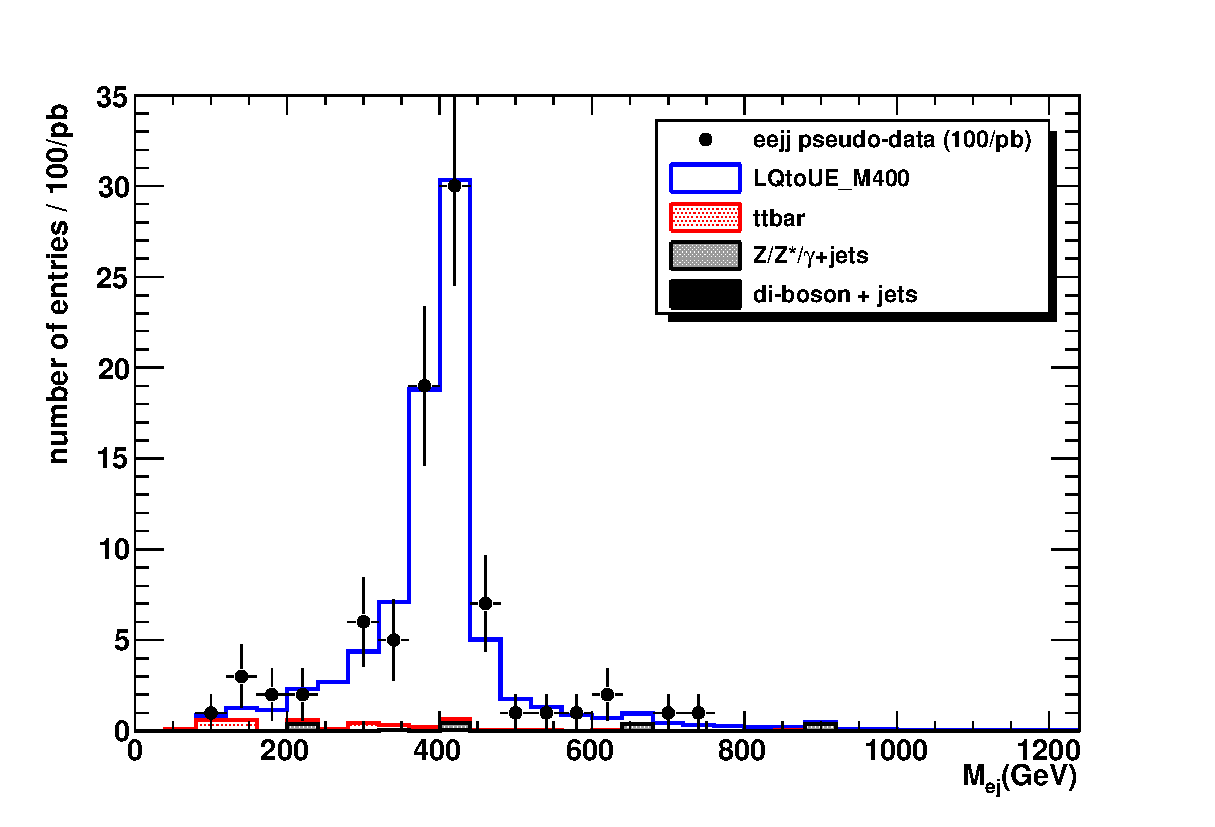
\includegraphics[width=1.1\linewidth]{plots/Mej_eejj_LQ400_100pb_LinScale.eps}
\caption{\label{fig:ejmass}
Invariant mass of the $LQ$ and the $\bar{LQ}$ candidates in events
with two electrons and two jets (points) with prediction from
SM background sources (lines).
The electron-jet pairing that
gives the minimum difference between the two candidates is used.}
\end{figure}


For setting upper limits in the absence of the leptoquark signal, 
the Bayesian approach\cite{bib:bayes} is used, with systematic uncertainties
marginalized as nuisance parameters.
The systematic uncertainties for the backgrounds are dominated by
the number of events in the control samples.  Systematic uncertainties
on the signal include (in order of importance)
the uncertainty on the integrated luminosity ($\pm 10$\%), uncertainties
on the production cross section {$\pm$ 10\%), 
jet energy scale, electron
identification efficieicies.

Limits as a function of $\beta$ are given in Figure ~\ref{fig:finalresult}
along with the expected limit.  As you can see, our limit is 
worse than expected, and we may expect interesting things in the future.


\begin{figure}[tbp]
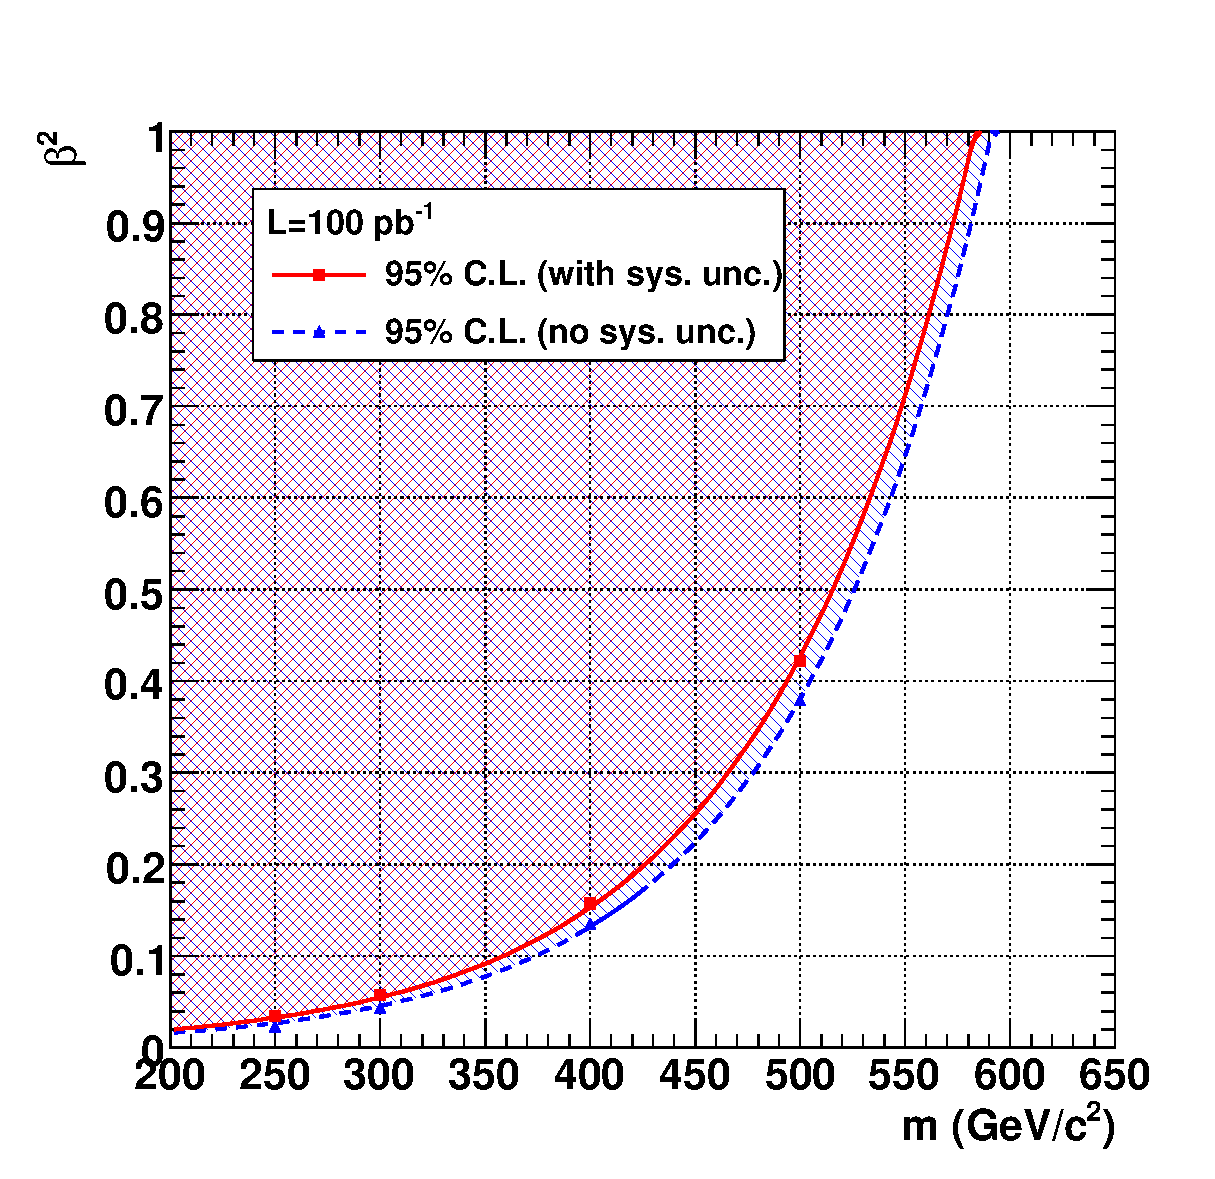
\includegraphics[width=1.1\linewidth]{plots/beta2_vs_m_excl.eps}
\caption{\label{fig:finalresult}
Observed and expected 95\% confidence-level limit on the 
mass of a first generation scalar LQ as a function of 
the LQ branching fraction to an electron and a jet, $\beta$.}
\end{figure}



In conclusion, we have presented search for first generation LQ.
Our data is in good agreement with the expectations from SM
processes.  Our limit on the mass of a scalar leptoquark
with $\beta=1$ is 535 \mgev.

We thank the staffs at CERN and collaborating institutions, and
acknowledge support from the
%
Austrian Federal Ministry of Science and Research; FNRS and FWO (Belgium); 
CNPq and FAPERJ (Brazil); 
Bulgarian Ministry of Education and Science; 
CERN; 
CAS and NSFC (China); 
Croatian Ministry of Science and Technology; 
University of Cyprus; 
Estonian Academy of Sciences and NICPB; 
Academy of Finland, Finish Ministry of Education and Helsinki Institute of Physics; 
CEA and CNRS/IN2P3 (France); 
BMBF and DESY (Germany); 
General Secretariat for Research and Technology (Greece); 
NKTH (Hungary); 
DAE and DST (India); 
IPM (Iran); 
UCD (Ireland); 
INFN (Italy); 
KICOS (Korea); 
CINVESTAV (Mexico); 
PAEC (Pakistan); 
State Commission for Scientific Research (Poland); 
FCT (Portugal); 
JINR (Armenia, Belarus, Georgia, Ukraine, Uzbekistan),
Ministry of Education and Science of the Russian Federation, 
Russian Federal Agency of Atomic Energy; 
Ministry of Science and Environmental Protection of the Republic of Serbia; 
Oficina de Ciencia y Tecnologia (Spain); 
ETHZ, PSI, University of Zurich (Switzerland); 
National Science Council (Taipei); 
TUBITAK and TAEK (Turkey); 
STFC (United Kingdom); 
DOE and NSF (USA).

\begin{thebibliography}{99}


\bibitem{bib:sm} S. Glashow, Nucl. Phys. {\bf 22}, 579 (1961);
 S. Weinbert, Phys. Rev. Lett. {\bf 19}, 1264 (1967);
 A. Salam, in {\it Elementary Particle Theory}, edited
by N. Svartholm (Almqvist and Wiksells, Stockholm, 1969), p. 367;
 W. Bardeen, H. Fritzsch, and M. Gell-Mann, in {\it Scale and
Conformal Symmetry in Hadron Physics}, edited by
R. Gatto (Wiley, New York, 1973), p. 139;
D. Gross and F. Wilczek, Phys. Rev. D {\bf 8}, 3633 (1973);
S. Weinbert, Phys. Rev. Lett. {\bf 31}, 494 (1973).

\bibitem{bib:patisalam} J.C. Pati and A. Salam, Phys. Rev. D {\bf 10}, 275 
(1974). 

\bibitem{bib:technicolor} S. Dimopoulos and L. Susskind, Nucl. Phys. B {\bf 155} (1979); S. Dimopoulos, Nucl. Phys. B {\bf 168} (1980); E. Eichten and K. Lane, Phys. Lett. B {\bf 90} (1980).

\bibitem{bib:composite}
W. Buchmu�ller and D. Wyler, Phys. Lett. B {\bf 177}, 377 (1986).

\bibitem{bib:e6} V.D. Angelopoulos {\it et al.}, Nucl. Phys. B {\bf 292} (1987).

\bibitem{bib:lqconst} W. Buchmuller, R. Ruckl, and D. Wyler, 
Phys. Lett. B {\bf 191}, 442 (1987); {\bf 448}, 320(e) (1999).


\bibitem{bib:cdflq} D. Acosta {\it et al.} [CDF Collaboration],
Phys. Rev. D {\bf 72}, 051107 (2005).

\bibitem{bib:d0lq} V.M. Abazov {\it et al.} [D0 Collaboration],
Phys. Rev. D {\bf 71}, 071104(R) (2005).

\bibitem{bib:kramer1} M. Kramer, arXiv:0411038.
\bibitem{bib:kramer2} M. Kramer, private communication.

\bibitem{bib:geo} CMS uses a cylindrical coordinate system with the z axis 
running along the beam axis.  The 
angles $\theta$ and $\phi$ are the polar and azimuthal angles, respectively. 
Pseudorapidity is defined as $\eta = -ln[tan(\theta/2)]$
where $\theta$ is measured 
with respect to the interaction vertex. In the massless limit, $\eta$ is 
equivalent to the rapidity $y=(1/2)ln[(E+p_z)/(E-p_z)]$.

\bibitem{bib:pythia} pythia reference

\bibitem{bib:geant} Application Software Group, 
CERN Program Library Long Writeup, W5013.

\bibitem{bib:madgraph} madgraph reference


\bibitem{bib:cmsjinst} S. Chatrchyan {\it et al.}, JINST {\bf 3} S08004.

\bibitem{bib:lumi} paper on luminosity determination

\bibitem{bib:cmseid} paper on cms electron id
\bibitem{bib:cmsjetid} paper on cms jet id 
\bibitem{bib:cmsmuonid} paper on cms muon id

\bibitem{bib:bayes} C. Amsler {\it et al.}, 
Physics Letters B {\bf 667}, 1 (2008), section 32.3.1.

\end{thebibliography}


